\documentclass[a4paper,11pt]{article}

\usepackage[utf8]{inputenc}
\usepackage[english, main=english]{babel}
\usepackage[autostyle]{csquotes}
\usepackage{geometry}
\usepackage{tikz}
\usetikzlibrary{positioning} 
\usetikzlibrary{fit}
\usetikzlibrary{calc}
\usetikzlibrary{external} % cache tikz figures
\tikzexternalize[
    shell escape={-shell-escape\space-output-directory=build},
]
\usepackage{pgfplots}
\usepackage{amsmath,amssymb,amsthm,bm}
\usepackage{siunitx}
\usepackage[ruled]{algorithm2e}
\usepackage{subcaption}


% theorem styles
\newtheorem{definition}{Definition}[section]

% math operators
\DeclareMathOperator*{\argmax}{arg\,max}
\DeclareMathOperator*{\argmin}{arg\,min}
\newcommand{\norm}[1]{\left\lVert#1\right\rVert}


\geometry{
 a4paper,
 total={170mm,240mm},
 left=20mm,
 top=30mm,
 }


\title{\vspace{-10mm}Tikplotlib Example}



\begin{document}
\maketitle

\begin{figure}[h]
\begin{minipage}[b]{0.49\textwidth}
    % This file was created with tikzplotlib v0.10.1.
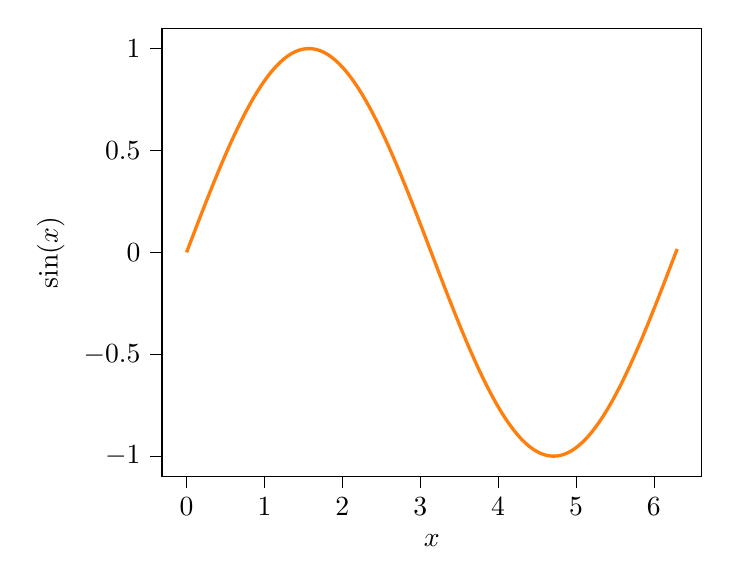
\begin{tikzpicture}

\definecolor{darkgray176}{RGB}{176,176,176}
\definecolor{darkorange25512714}{RGB}{255,127,14}

\begin{axis}[
tick align=outside,
tick pos=left,
x grid style={darkgray176},
xlabel={\(\displaystyle x\)},
xmin=-0.315, xmax=6.615,
xtick style={color=black},
y grid style={darkgray176},
ylabel={\(\displaystyle \sin(x)\)},
ymin=-1.09990860865177, ymax=1.09976911527703,
ytick style={color=black}
]
\addplot [very thick, darkorange25512714]
table {%
0 0
0.05 0.0499791692706783
0.1 0.0998334166468282
0.15 0.149438132473599
0.2 0.198669330795061
0.25 0.247403959254523
0.3 0.29552020666134
0.35 0.342897807455451
0.4 0.389418342308651
0.45 0.43496553411123
0.5 0.479425538604203
0.55 0.522687228930659
0.6 0.564642473395035
0.65 0.60518640573604
0.7 0.644217687237691
0.75 0.681638760023334
0.8 0.717356090899523
0.85 0.751280405140293
0.9 0.783326909627484
0.95 0.813415504789374
1 0.841470984807897
1.05 0.867423225594017
1.1 0.891207360061435
1.15 0.912763940260521
1.2 0.932039085967226
1.25 0.948984619355586
1.3 0.963558185417193
1.35 0.975723357826659
1.4 0.98544972998846
1.45 0.992712991037588
1.5 0.997494986604054
1.55 0.999783764189357
1.6 0.999573603041505
1.65 0.996865028453919
1.7 0.991664810452468
1.75 0.983985946873937
1.8 0.973847630878195
1.85 0.9612752029753
1.9 0.946300087687414
1.95 0.928959715003869
2 0.909297426825682
2.05 0.887362368633375
2.1 0.863209366648874
2.15 0.836898790798498
2.2 0.80849640381959
2.25 0.778073196887921
2.3 0.74570521217672
2.35 0.711473352790844
2.4 0.675463180551151
2.45 0.637764702134504
2.5 0.598472144103956
2.55 0.557683717391417
2.6 0.515501371821464
2.65 0.472030541289882
2.7 0.42737988023383
2.75 0.381660992052332
2.8 0.334988150155905
2.85 0.287478012342544
2.9 0.239249329213982
2.95 0.190422647361027
3 0.141120008059867
3.05 0.0914646422324368
3.1 0.0415806624332905
3.15 -0.00840724736714906
3.2 -0.0583741434275801
3.25 -0.108195134530108
3.3 -0.157745694143249
3.35 -0.2069019716734
3.4 -0.255541102026832
3.45 -0.303541512708429
3.5 -0.35078322768962
3.55 -0.39714816728596
3.6 -0.442520443294852
3.65 -0.4867866486557
3.7 -0.529836140908493
3.75 -0.571561318742344
3.8 -0.611857890942719
3.85 -0.650625137065167
3.9 -0.687766159183974
3.95 -0.723188124086512
4 -0.756802495307928
4.05 -0.788525254426195
4.1 -0.818277111064411
4.15 -0.845983701075447
4.2 -0.871575772413588
4.25 -0.894989358228583
4.3 -0.916165936749455
4.35 -0.935052577558449
4.4 -0.951602073889516
4.45 -0.965773060620639
4.5 -0.977530117665097
4.55 -0.986843858503237
4.6 -0.993691003633464
4.65 -0.998054438758879
4.7 -0.999923257564101
4.75 -0.999292788975378
4.8 -0.99616460883584
4.85 -0.990546535966713
4.9 -0.982452612624332
4.95 -0.971903069401821
5 -0.958924274663139
5.05 -0.943548668635906
5.1 -0.925814682327732
5.15 -0.905766641468704
5.2 -0.883454655720153
5.25 -0.858934493426592
5.3 -0.832267442223901
5.35 -0.803520155852155
5.4 -0.772764487555987
5.45 -0.740077310488894
5.5 -0.705540325570392
5.55 -0.669239857276261
5.6 -0.631266637872321
5.65 -0.591715580631009
5.7 -0.550685542597637
5.75 -0.508279077499258
5.8 -0.464602179413757
5.85 -0.419764017839859
5.9 -0.373876664830236
5.95 -0.327054814869741
6 -0.279415498198926
6.05 -0.231077788299391
6.1 -0.182162504272095
6.15 -0.132791908852517
6.2 -0.0830894028174964
6.25 -0.0331792165475568
6.3 0.0168139004843506
};
\end{axis}

\end{tikzpicture}

    \vspace{-1cm}
\end{minipage}
\hfill
\begin{minipage}[b]{0.49\textwidth}
    % This file was created with tikzplotlib v0.10.1.
\begin{tikzpicture}

\definecolor{darkgray176}{RGB}{176,176,176}

\begin{axis}[
colorbar,
colorbar style={ylabel={}},
colormap/viridis,
point meta max=0.999887918747638,
point meta min=-0.999923257564101,
tick align=outside,
tick pos=left,
x grid style={darkgray176},
xlabel={\(\displaystyle x\)},
xmin=-0.025, xmax=6.325,
xtick style={color=black},
y grid style={darkgray176},
ylabel={\(\displaystyle y\)},
ymin=-0.025, ymax=6.325,
ytick style={color=black}
]
\addplot graphics [includegraphics cmd=\pgfimage,xmin=-0.025, xmax=6.325, ymin=-0.025, ymax=6.325] {plots/2d_plot-000.png};
\end{axis}

\end{tikzpicture}

    \vspace{-1cm}
\end{minipage}
\caption{1D plot (left) and 2D plot (right).}
\label{fig:example_plots}
\end{figure}

\end{document}
